\documentclass[aspectratio=169,10pt]{beamer}

\usetheme{Madrid}
\usecolortheme{seahorse}

\usepackage[utf8]{inputenc}
\usepackage{amsmath, amssymb, amsfonts}
\usepackage{mathtools}
\usepackage{listings}
\usepackage{xcolor}
\usepackage{graphicx}
\usepackage{tikz}

\graphicspath{{figures/}}

% Define colors for code
\definecolor{codegreen}{rgb}{0,0.6,0}
\definecolor{codegray}{rgb}{0.5,0.5,0.5}
\definecolor{codepurple}{rgb}{0.58,0,0.82}
\definecolor{backcolour}{rgb}{0.95,0.95,0.92}

\lstdefinestyle{pythonstyle}{
    backgroundcolor=\color{backcolour},
    commentstyle=\color{codegreen}\itshape,
    keywordstyle=\color{codepurple}\bfseries,
    numberstyle=\tiny\color{codegray},
    stringstyle=\color{codepurple},
    basicstyle=\ttfamily\scriptsize,
    breakatwhitespace=false,
    breaklines=true,
    captionpos=b,
    keepspaces=true,
    numbers=left,
    numbersep=5pt,
    showspaces=false,
    showstringspaces=false,
    showtabs=false,
    tabsize=2,
    frame=single,
    rulecolor=\color{black}
}

\lstset{style=pythonstyle}

% Set footer
\setbeamertemplate{footline}[frame number]

% Title info
\title{Common Fixed Points \& Sequences}
\subtitle{Chapter 5e: Pathak's Fixed Point Theory}
\author{Nonlinear Analysis \& Fixed Point Theory}
\date{2024}

\begin{document}

% Title slide
\frame{\titlepage}

% Table of contents
\begin{frame}{Overview}
    \tableofcontents
\end{frame}

% ============================================================================
\section{5.5 Common Fixed Point Theorems}
% ============================================================================

\begin{frame}{Section 5.5: Common Fixed Point Theorems}
    \begin{itemize}
        \item \textbf{Definition}: A point $u \in X$ is a \alert{common fixed point} of mappings $f$ and $g$ if:
        \[
            f(u) = u \quad \text{and} \quad g(u) = u
        \]

        \item \textbf{Key Question}: When do two (or more) mappings have a common fixed point?

        \item \textbf{History}:
        \begin{itemize}
            \item Markov (1936): First result on common fixed points
            \item Kakutani (1938): Direct proof using Tychonoff's theorem
            \item Subsequent extensions for families of mappings
        \end{itemize}

        \item \textbf{Applications}:
        \begin{itemize}
            \item Systems of equations
            \item Simultaneous fixed points of operators
            \item Optimization problems
        \end{itemize}
    \end{itemize}
\end{frame}

\begin{frame}{Common Fixed Points Visualization}
    \centering
    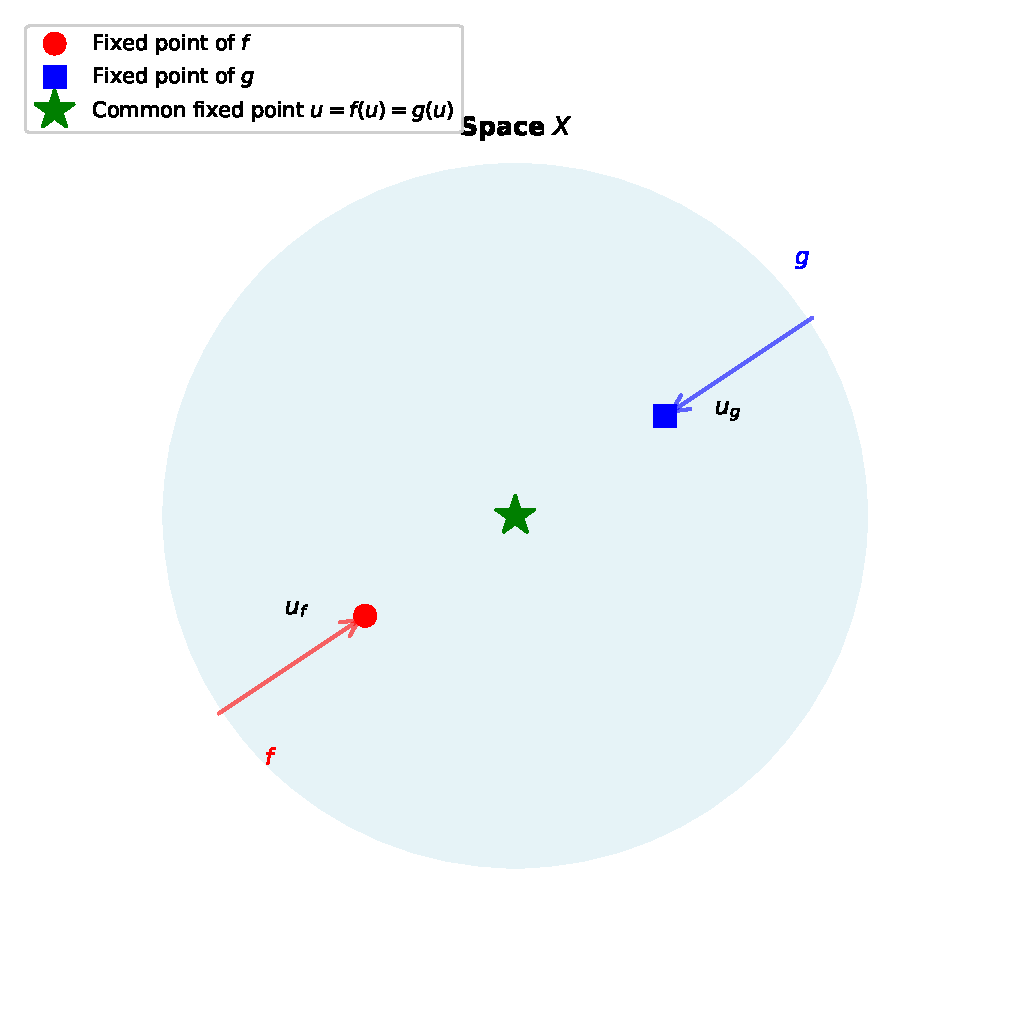
\includegraphics[width=0.85\textwidth]{fig_common_fixed_points.pdf}
\end{frame}

\begin{frame}{Theorem 5.118: Two Mappings with Weak Compatibility}
    \textbf{Theorem 5.118} (Weakly Compatible Mappings): Let $(X, d)$ be a b-metric space and let $f, g: X \to X$ be mappings satisfying:

    \medskip

    \[
    d(f(x_1, x_2, \ldots, x_k), g(x_2, x_3, \ldots, x_{k+1})) \leq \lambda\phi(d(gx_1, gx_2), \ldots)
    \]

    where $\lambda \in (0, \frac{1}{s})$, $s \geq 1$, and $g(X)$ is complete.

    \medskip

    If $f$ and $g$ are \textbf{weakly compatible}, then:
    \begin{enumerate}
        \item $C(f, g) \neq \emptyset$ (common fixed point exists)
        \item Sequences defined by iteration converge to the common fixed point
        \item The common fixed point is unique
    \end{enumerate}

    \medskip
    \small
    \textbf{Definition (Weak Compatibility)}: $f$ and $g$ are weakly compatible if they commute at their common fixed points.
\end{frame}

\begin{frame}{Example 5.47: Concrete Common Fixed Points}
    \textbf{Example 5.47}: Let $X = \mathbb{R}$, $d(x,y) = |x-y|^3$, $s=4$. Define:

    \[
    f(x, y) = \frac{x^2 + y^2}{13} + \frac{18}{13}, \quad g(x) = x^2 - 2
    \]

    \medskip

    \textbf{Verification}:
    \begin{itemize}
        \item Check condition (5.115): $d(f(x,y), f(y,z)) \leq \lambda \phi(d(gx, gy), \ldots)$
        \item With $\lambda = \frac{8}{13^3} \in (0, \frac{1}{4})$
        \item Functions $f$ and $g$ commute at fixed points
    \end{itemize}

    \medskip

    \textbf{Result}: Common fixed point is $u = 2$, where:
    \[
    f(-1, -1) = 1 = (-1)^2 - 2, \quad f(1, 1) = 2 = 2^2 - 2
    \]
\end{frame}

\begin{frame}{Example 5.47 Visualization}
    \centering
    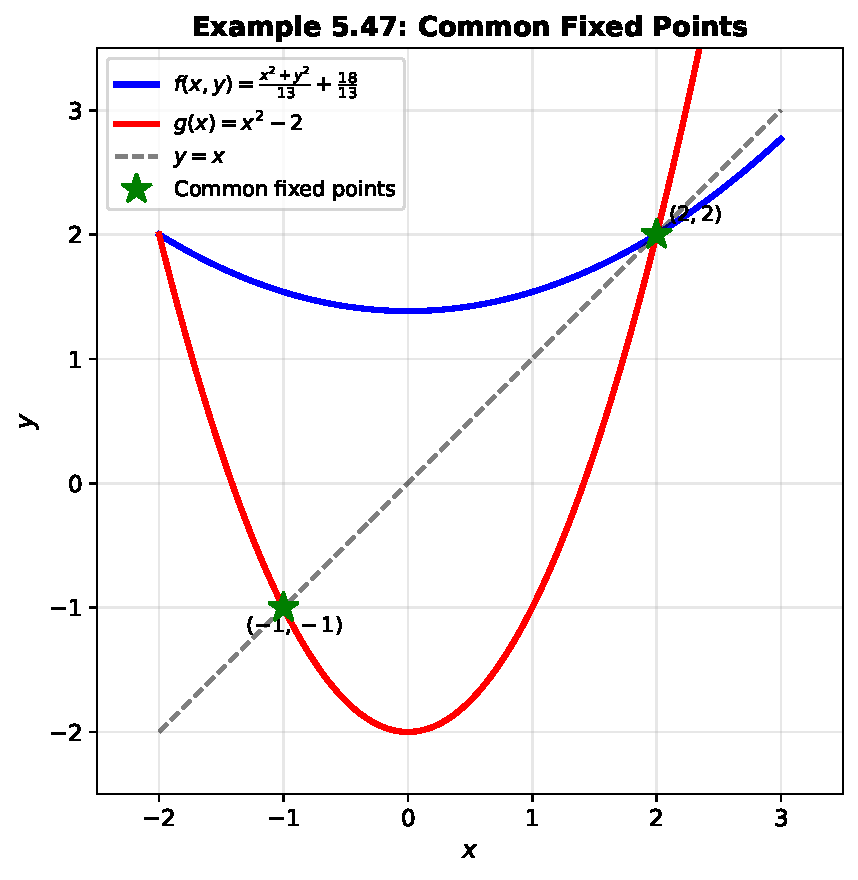
\includegraphics[width=0.85\textwidth]{fig_example_547.pdf}
\end{frame}

\subsection{5.5.2 Families of Mappings}

\begin{frame}{5.5.2: Common Fixed Points of Family of Mappings}
    \textbf{Definition 5.67}: Let $K$ be a convex subset of a normed linear space $X$ and let $F$ be a self-mapping of $K$. $F$ is \alert{affine mapping} if:

    \[
    F(\alpha x + (1-\alpha)y) = \alpha F x + (1-\alpha) F y \quad \forall x, y \in K, \, 0 < \alpha < 1
    \]

    \medskip

    \textbf{Definition 5.68}: A family $\mathcal{F}$ of linear mappings is \alert{equicontinuous on subset $K$} if:

    For every neighborhood $V$ of the origin and $\delta > 0$, there exists neighborhood $U$ such that if $x - y \in U$, then $F(x) - F(y) \in V$ for all $F \in \mathcal{F}$.

    \medskip

    \textbf{Key Theorem (Markov-Kakutani 1936-1938)}:

    Compact convex subset + commuting affine maps $\Rightarrow$ non-empty common fixed point set
\end{frame}

\begin{frame}{Theorem 5.120: Markov-Kakutani Theorem}
    \textbf{Theorem 5.120} (Markov-Kakutani): Let $K$ be a compact convex subset of a normed linear space $X$. Let $\mathcal{F}$ be a commuting family of continuous affine mappings which map $K$ into itself.

    \medskip

    Then there exists a point $u \in K$ such that $Fu = u$ for each $F \in \mathcal{F}$.

    \medskip

    \textbf{Proof Strategy}:
    \begin{enumerate}
        \item Define $F_n(K) = n^{-1}(I + F + \cdots + F^{n-1})(K)$
        \item Show $F_n(K)$ are convex and compact
        \item Finite subfamily has non-void intersection (compactness)
        \item Common intersection point is fixed by all $F \in \mathcal{F}$
    \end{enumerate}
\end{frame}

\begin{frame}{Theorem 5.121: Kakutani's Equicontinuous Extension}
    \textbf{Theorem 5.121} (Kakutani [302]): Let $K$ be a compact convex subset of a normed linear space $X$, and let $\mathcal{F}$ be a group of affine mappings which is equicontinuous on $K$ and such that $F(K) \subset K$ for all $F \in \mathcal{F}$.

    \medskip

    Then there exists a point $u \in K$ such that $Fu = u$ for all $F \in \mathcal{F}$.

    \medskip

    \textbf{Key Differences from Theorem 5.120}:
    \begin{itemize}
        \item Requires equicontinuity instead of commutativity
        \item Group structure (all mappings invertible)
        \item More general setting
    \end{itemize}
\end{frame}

\begin{frame}{Theorems 5.122-5.129: Nonexpansive Mappings}
    \textbf{Theorem 5.122} (Ryll-Nadzewski [532]): Extension for semigroups of nonexpanding mappings

    \textbf{Theorem 5.123} (de Marr [165]): Family of commuting nonexpansive mappings on compact convex Banach space subset has common fixed point.

    \textbf{Theorem 5.124} (Belluce-Kirk [46]): Closed, bounded, convex subset + commuting nonexpansive family $\Rightarrow$ common fixed point

    \textbf{Theorem 5.125} (Weakly Compact Generalization): For weakly compact convex subsets of strictly convex Banach spaces

    \textbf{Theorem 5.126} (Browder [96]): Uniformly convex Banach spaces

    \textbf{Theorem 5.127}: Multivalued mappings with generalized Kannan-Reich condition

    \textbf{Theorem 5.128}: Sequences of self-mappings with generalized Kannan-Reich type condition

    \textbf{Theorem 5.129}: Continuous function $\phi$ in multiple variables
\end{frame}

\begin{frame}{Iteration Schemes for Families}
    \textbf{Theorem 5.130-5.131}: Iteration schemes converging to common fixed points

    For finite family $\{F_i\}_{i=1}^k$ of nonexpansive mappings on compact convex Banach space, define:

    \[
    U_0 = I \quad \text{(identity mapping)}
    \]
    \[
    U_r = (1-\alpha)I + \alpha F_r U_{r-1}, \quad r = 1, 2, \ldots, k
    \]

    \medskip

    \textbf{Results}:
    \begin{itemize}
        \item For $0 < \alpha < 1$, sequence $\{U_n^k x\}$ converges strongly to common fixed point
        \item Weak convergence in Hilbert/reflexive spaces
        \item Iterations reduce to solving systems of equations: $x - T_i x = f_i$
    \end{itemize}

    \medskip

    \textbf{Remark 5.49}: Application to systems of equations in Banach spaces
\end{frame}

\begin{frame}{Family of Mappings Visualization}
    \centering
    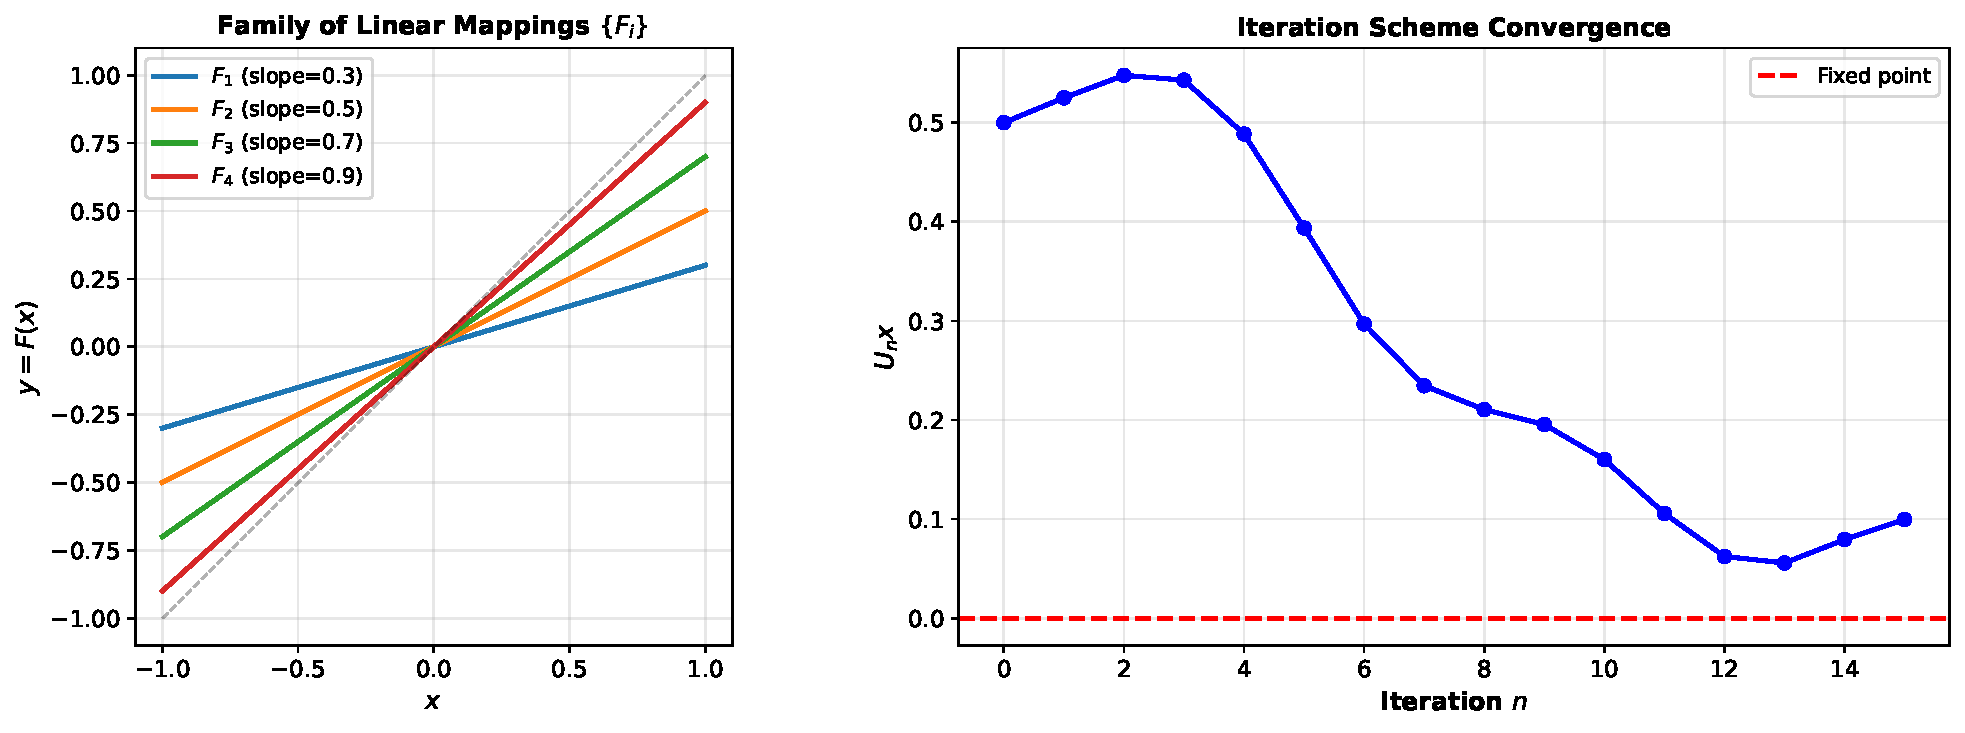
\includegraphics[width=0.95\textwidth]{fig_family_mappings.pdf}
\end{frame}

% ============================================================================
\section{5.6 Sequences of Contractions}
% ============================================================================

\begin{frame}{Section 5.6: Sequences of Contractions}
    \textbf{Main Question}: If we have a sequence of contraction mappings $\{T_n\}$ converging to a mapping $T$, does the sequence of fixed points converge to the fixed point of $T$?

    \medskip

    \textbf{Two Types of Convergence}:
    \begin{enumerate}
        \item \textbf{Pointwise Convergence}: $\lim_{n \to \infty} T_n x = T x$ for each $x$
        \item \textbf{Uniform Convergence}: $\lim_{n \to \infty} d(T_n x, T x) = 0$ uniformly
    \end{enumerate}

    \medskip

    \textbf{Key Results}:
    \begin{itemize}
        \item Bonsal [64]: Fixed point continuity for contractions
        \item Nadler Jr. [417, 416]: Behavior of fixed points for set-valued maps
        \item Conditions for convergence of fixed point sequences
    \end{itemize}
\end{frame}

\begin{frame}{Theorem 5.133: Contraction Sequences (Bonsal)}
    \textbf{Theorem 5.133} (Bonsal [64]): Let $(X, d)$ be a complete metric space, and let $T$ and $T_n$ ($n = 1, 2, \ldots$) be contraction mappings of $X$ into itself with the same Lipschitz constant $k < 1$, with fixed points $u$ and $u_n$, respectively.

    Suppose that $\lim_{n \to \infty} T_n x = T x$ for every $x \in X$.

    \medskip

    Then: $\lim_{n \to \infty} u_n = u$

    \medskip

    \textbf{Proof Sketch}:
    \[
    d(u_r, T_r^n x_0) \leq \frac{k^n}{1-k} d(T x_0, x_0)
    \]
    Combined with pointwise convergence gives convergence of fixed points.
\end{frame}

\begin{frame}{Contraction Convergence Visualization}
    \centering
    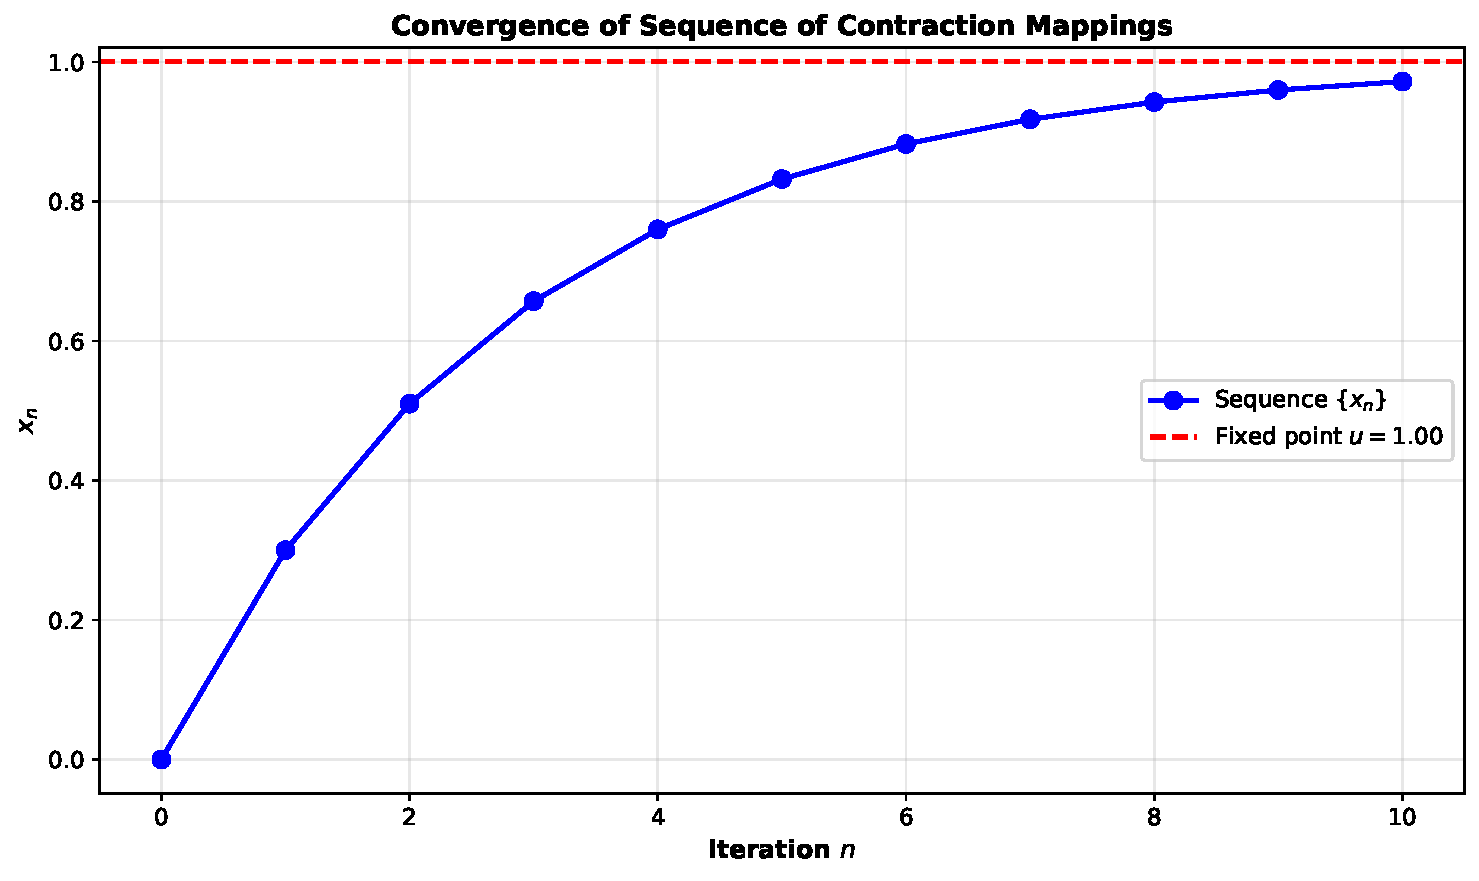
\includegraphics[width=0.85\textwidth]{fig_contraction_convergence.pdf}
\end{frame}

\begin{frame}{Theorem 5.134-5.135: Uniform Convergence}
    \textbf{Theorem 5.134}: Let $(X, d)$ be a metric space. Let $T_i: X \to X$ be a mapping with at least one fixed point $x_i$ for each $i = 1, 2, \ldots$, and let $T_0: X \to X$ be a contraction mapping with fixed point $x_0$.

    If the sequence $\{T_i\}$ converges uniformly to $T_0$, then the sequence $\{x_i\}$ converges to $x_0$.

    \medskip

    \textbf{Theorem 5.135}: Let $(X, d)$ be a locally compact metric space. Let $T_i: X \to X$ be a contraction mapping with fixed point $x_i$ for each $i = 1, 2, \ldots$, and let $T_0: X \to X$ be a contraction mapping with fixed point $x_0$.

    If the sequence $\{T_i\}$ is equicontinuous and converges pointwise to $T_0$, then the sequence $\{x_i\}$ converges to $x_0$.
\end{frame}

\begin{frame}{Theorem 5.136: Finite Dimensionality Characterization}
    \textbf{Theorem 5.136} (Nadler Jr. [417]): A separable or reflexive Banach space is finite dimensional if and only if, whenever for a pointwise convergent sequence of contraction mappings, the sequence of fixed point converges to the fixed point of the pointwise limit mapping.

    \medskip

    \textbf{Corollary}: This provides a topological characterization of finite dimensional spaces through fixed point behavior.

    \medskip

    \textbf{Interpretation}:
    \begin{itemize}
        \item In finite dimensions: convergence of mappings $\Rightarrow$ convergence of fixed points
        \item In infinite dimensions: may fail without additional conditions
        \item Shows fundamental difference between finite and infinite dimensional spaces
    \end{itemize}
\end{frame}

\begin{frame}{Theorem 5.137-5.138: Multivalued Contractions}
    \textbf{Theorem 5.137} (Nadler Jr. [416]): Let $(X, d)$ be a complete metric space. Let $T_i: X \to \mathcal{K}(X)$ be multivalued contraction mappings with fixed point $x_i$ for each $i = 1, 2, \ldots$, and let $T_0: X \to \mathcal{K}(X)$ be a multivalued contraction mapping.

    \medskip

    If (i) each $T_i$ has Lipschitz constant $\eta < 1$, (ii) $\{T_i\}$ converges uniformly to $T_0$, or (iii) $(X, d)$ is locally compact and $\{T_i\}$ converges pointwise to $T_0$,

    then there is a subsequence $\{x_j\}$ that converges to a fixed point of $T_0$.

    \medskip

    \textbf{Theorem 5.138} (Markin [385]): For setvalued contractions with Hausdorff metric, fixed point sets converge in Hausdorff metric.
\end{frame}

\begin{frame}{Theorems 5.139-5.142: Weak Convergence}
    \textbf{Theorem 5.139} (Markin [386]): Weak convergence of fixed points for setvalued nonexpansive mappings in strictly convex Banach spaces with weakly continuous duality map

    \medskip

    \textbf{Definition 5.69}: A mapping $T: X \to X$ is of \alert{generalized Kannan-Reich type} if:
    \[
    d(Tx, Ty) \leq a_1 d(Tx, x) + a_2 d(Ty, y) + a_3 d(Ty, x) + a_4 d(Tx, y) + a_5 d(x, y)
    \]
    where $\sum_{i=1}^5 a_i < 1$ and $a_1 = a_2, a_3 = a_4$

    \medskip

    \textbf{Theorem 5.140}: Uniform convergence of Kannan-Reich type mappings preserves fixed points

    \textbf{Theorem 5.141}: Pointwise convergence with Kannan-Reich property

    \textbf{Theorem 5.142}: Multivalued mappings with similar generalized conditions
\end{frame}

\begin{frame}{Theorem 5.143: Husain-Sehgal Type Mappings}
    \textbf{Theorem 5.143}: Let $T$ and a sequence $\{T_n\}$ be self-mappings of a complete metric space $X$ such that $T_n \to T$ uniformly.

    Suppose for each $n \geq 1$, $T_n$ has a fixed point $x_n$ and $T$ is a mapping of \alert{Husain-Sehgal type}.

    \medskip

    If $u$ is the fixed point of $T$ and $\sup d(x_n, u) < \infty$, then $x_n \to u$.

    \medskip

    \textbf{Husain-Sehgal Type Condition}: Involves $(I - T)$ being J-monotone

    \medskip

    \textbf{Applications}:
    \begin{itemize}
        \item Differential equations with perturbations
        \item Stability of fixed points under approximation
        \item Numerical methods with rounding errors
    \end{itemize}
\end{frame}

\begin{frame}{Iteration Process Visualization}
    \centering
    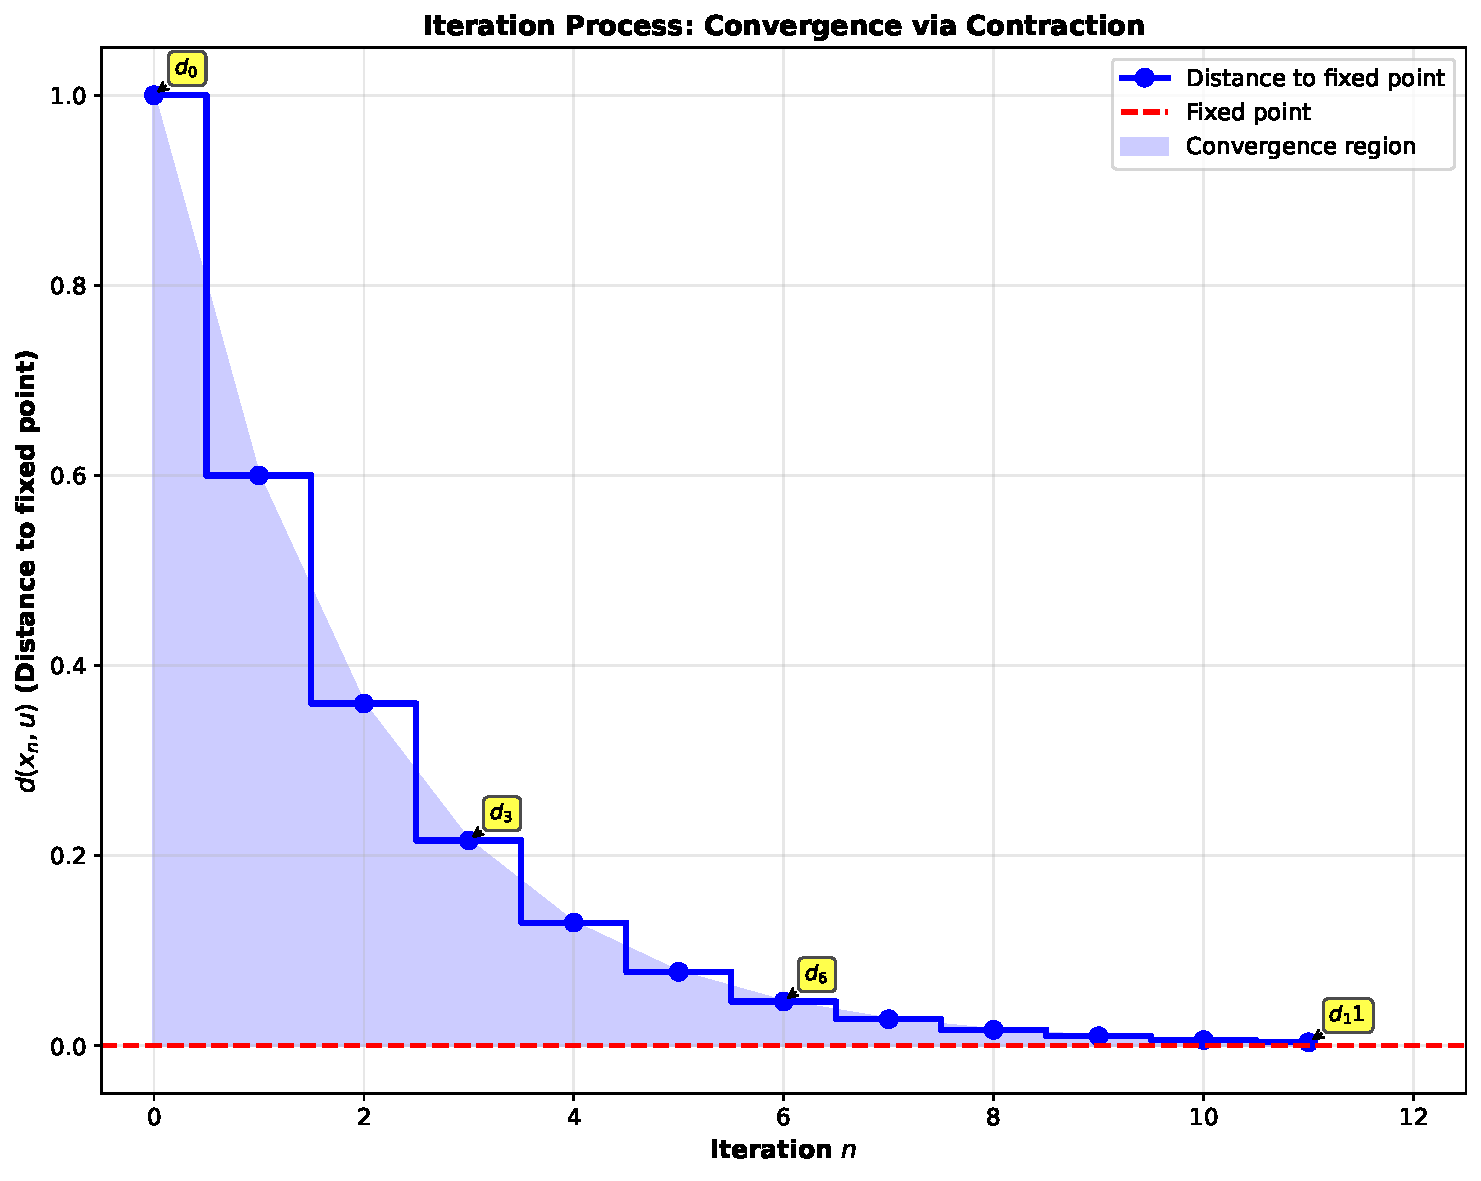
\includegraphics[width=0.85\textwidth]{fig_iteration_process.pdf}
\end{frame}

% ============================================================================
\section{5.7 Fixed Point Theorems in Ordered Banach Spaces}
% ============================================================================

\begin{frame}{Section 5.7: Ordered Banach Spaces}
    \textbf{Definition 5.70}: Let $X$ be a real Banach space. A set $K \subset X$ is a \alert{cone} if:
    \begin{enumerate}
        \item $K$ is closed
        \item If $u, v \in K$, then $\alpha u + \beta v \in K$ for all $\alpha, \beta \geq 0$
        \item $x, -x \in K \Rightarrow x = 0$
    \end{enumerate}

    \medskip

    \textbf{Definition 5.71}: A linear space $X$ is \alert{partially ordered} by relation $\leq$ if:
    \begin{enumerate}
        \item $x \leq y \Rightarrow tx \leq ty$ for $t \geq 0$
        \item $x \leq y$ and $y \leq x$ implies $x = y$
        \item $x_1 \leq y_1$ and $x_2 \leq y_2$ implies $x_1 + x_2 \leq y_1 + y_2$
        \item $x \leq y$ and $y \leq z$ implies $x \leq z$
    \end{enumerate}

    In Banach space: $x \leq y$ iff $y - x \in K$
\end{frame}

\begin{frame}{Cone Ordering Visualization}
    \centering
    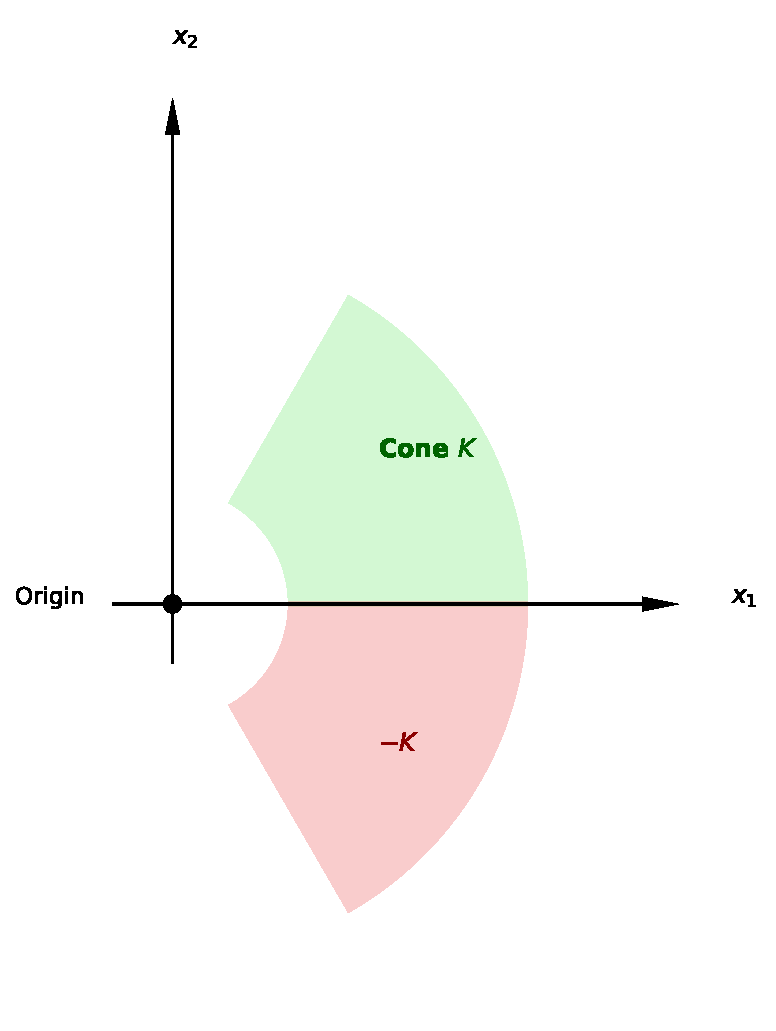
\includegraphics[width=0.85\textwidth]{fig_cone_ordering.pdf}
\end{frame}

\begin{frame}{Additional Concepts in Ordered Banach Spaces}
    \textbf{Definition 5.72}: An operator $F: X \to X$ is:
    \begin{itemize}
        \item \alert{Isotone (increasing)}: $x \leq y \Rightarrow Fx \leq Fy$
        \item \alert{Strictly increasing}: $x < y \Rightarrow Fx < Fy$ (with interior property)
        \item \alert{Strongly increasing}: $\text{int }K \neq \emptyset$ and $x < y \Rightarrow F(y) - F(x) \in \text{int }K$
    \end{itemize}

    \medskip

    \textbf{Definition 5.73}: A cone $K$ is \alert{normal} if there exists $\delta > 0$ such that:
    \[
    \|e_1 + e_2\| \geq \delta, \quad \text{whenever } \|e_1\| = \|e_2\| = 1, \; e_1, e_2 \in K
    \]

    \textbf{Definition 5.74}: Space $X$ is \alert{regularly partially ordered} if each bounded monotonic sequence has a limit. A cone which generates regular partial ordering is called regular.
\end{frame}

\begin{frame}{Theorem 5.144: Normal Cones Characterization}
    \textbf{Theorem 5.144} (Krasnoselski [345]): Let $(X, K)$ be an ordered Banach space. The following are equivalent:
    \begin{enumerate}
        \item $K$ is normal
        \item Every order interval is bounded
        \item There exists an equivalent increasing norm on $X$
        \item The order convex hull of every bounded set is bounded
    \end{enumerate}

    \medskip

    \textbf{Example 5.48}: Space $C(X)$ of continuous functions on compact Hausdorff space $X$ with sup norm. Normal cone $C_+(X)$ of non-negative functions with non-empty interior.

    \medskip

    \textbf{Example 5.49}: $L_p(\Omega)$ spaces ($1 \leq p \leq \infty$) are ordered Banach spaces with natural ordering and normal cones.
\end{frame}

\begin{frame}{Applications of Ordered Banach Spaces}
    \textbf{Key Applications}:
    \begin{itemize}
        \item \textbf{Differential Equations}: Finding positive solutions via fixed points
        \item \textbf{Integral Equations}: Volterra-type equations with ordering
        \item \textbf{Optimization}: Ordered sequences for extremal problems
        \item \textbf{Partial Differential Equations}: Monotone methods
    \end{itemize}

    \medskip

    \textbf{Advantages of Ordered Framework}:
    \begin{itemize}
        \item Monotonicity structure simplifies analysis
        \item Allows comparison principles
        \item Constructs iterative sequences with known bounds
        \item Relates to physical constraints (non-negativity, etc.)
    \end{itemize}

    \medskip

    \textbf{Connection to Fixed Points}:

    Isotone operators on cones often have unique fixed points that can be approximated by monotone iteration schemes.
\end{frame}

\begin{frame}{Banach Spaces Structure}
    \centering
    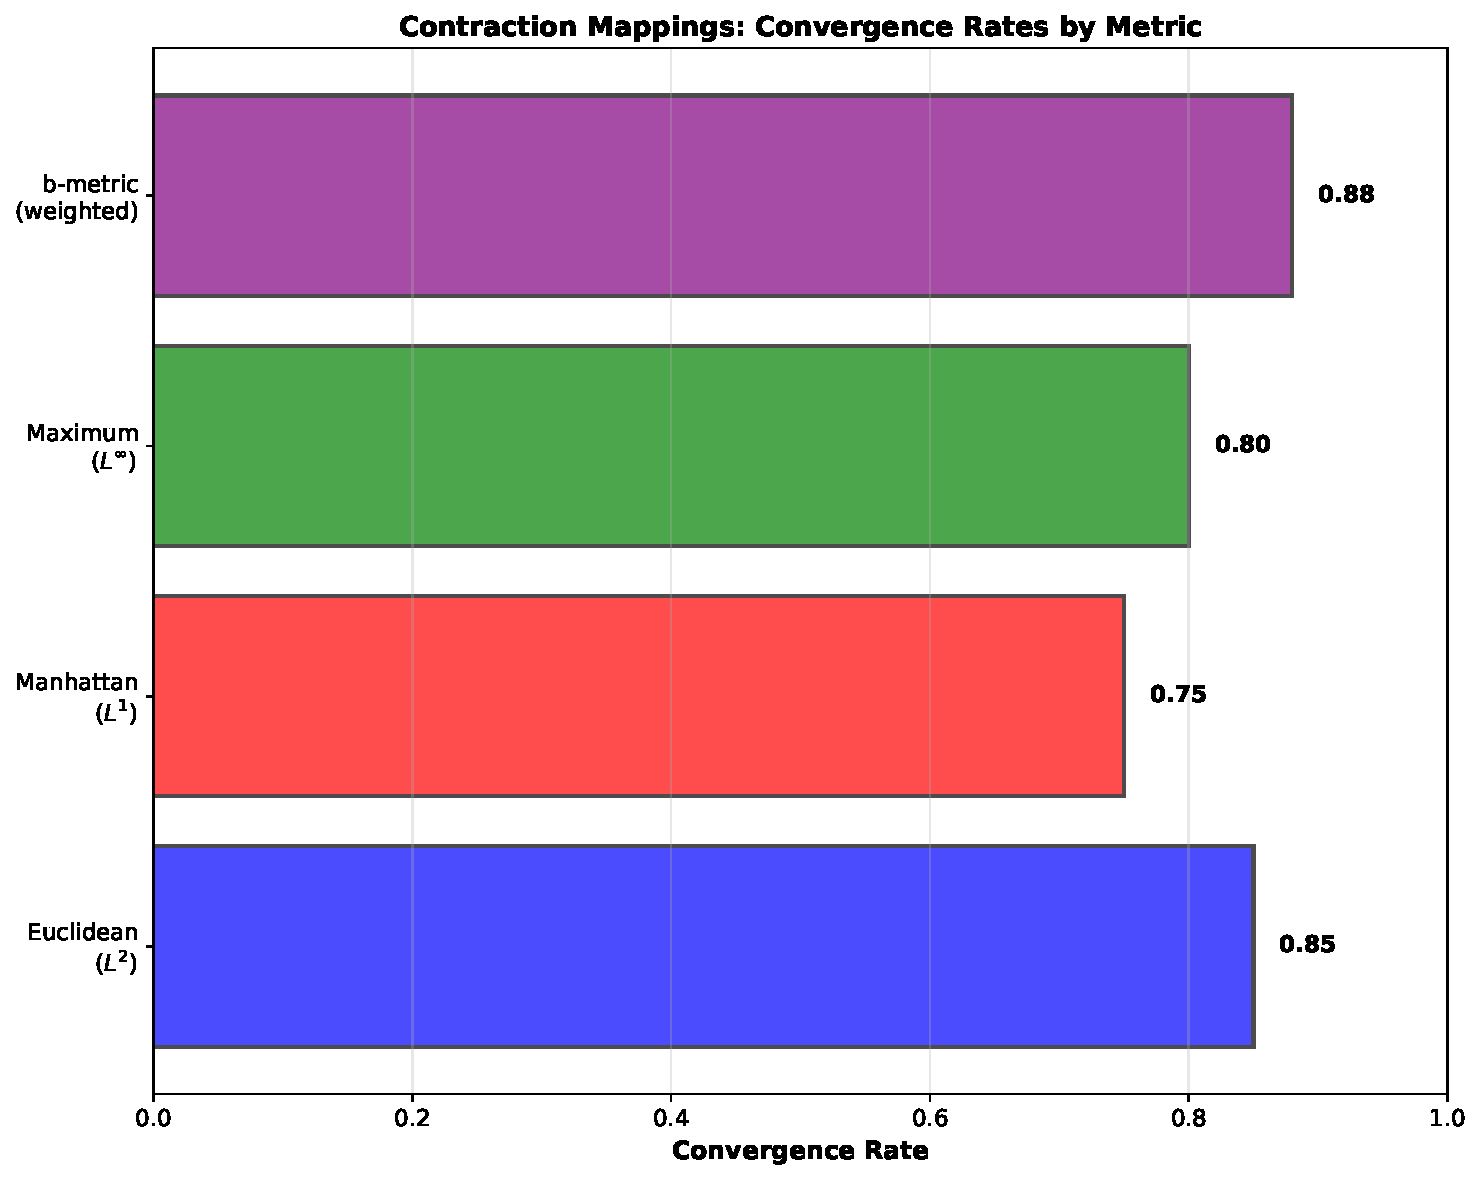
\includegraphics[width=0.85\textwidth]{fig_banach_metrics.pdf}
\end{frame}

% ============================================================================
\section{Summary and Connections}
% ============================================================================

\begin{frame}{Key Results Summary}
    \textbf{Section 5.5 - Common Fixed Points}:
    \begin{itemize}
        \item Weak compatibility + b-metric conditions $\Rightarrow$ unique common fixed point
        \item Markov-Kakutani: Compact convex + commuting affine maps
        \item Families of nonexpansive mappings on various Banach space types
    \end{itemize}

    \medskip

    \textbf{Section 5.6 - Sequences of Contractions}:
    \begin{itemize}
        \item Convergence of mapping sequences $\Rightarrow$ convergence of fixed points
        \item Uniform convergence sufficient; pointwise may require additional structure
        \item Finite dimensionality characterized by fixed point continuity
    \end{itemize}

    \medskip

    \textbf{Section 5.7 - Ordered Banach Spaces}:
    \begin{itemize}
        \item Cone-based partial ordering framework
        \item Normal cones and regular partial orderings
        \item Isotone operators have special fixed point properties
    \end{itemize}
\end{frame}

\begin{frame}{Uniqueness Results Summary}
    \centering
    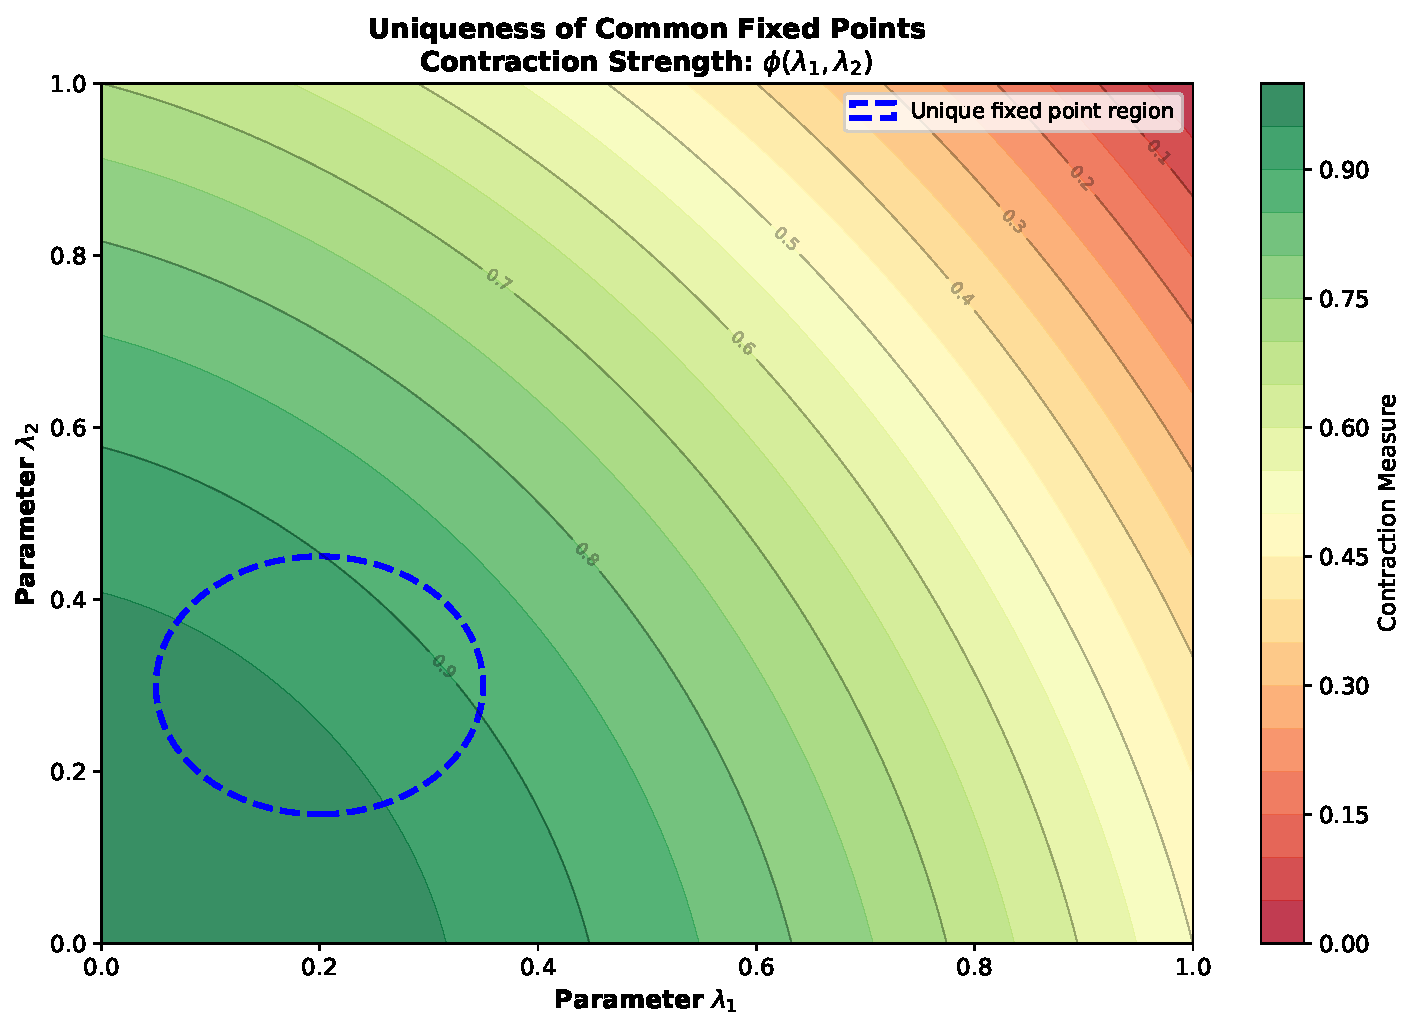
\includegraphics[width=0.85\textwidth]{fig_uniqueness.pdf}
\end{frame}

\begin{frame}{Comprehensive Outline}
    \textbf{Theorems 5.118-5.143}: Major Results

    \begin{tabular}{lll}
        \textbf{Theorem} & \textbf{Type} & \textbf{Setting} \\
        \hline
        5.118-5.119 & Weak compatibility & b-metric spaces \\
        5.120-5.121 & Families (affine) & Compact convex \\
        5.122-5.129 & Nonexpansive families & Banach spaces \\
        5.130-5.132 & Iteration schemes & Convex Banach spaces \\
        \hline
        5.133-5.135 & Contraction sequences & Complete metric \\
        5.136 & Finite dimension & Banach spaces \\
        5.137-5.142 & Multivalued/Kannan-Reich & General \\
        5.143 & Husain-Sehgal type & Complete metric \\
        \hline
        5.144 & Normal cones & Ordered Banach \\
    \end{tabular}

    \medskip

    \textbf{Common Theme}: Contraction-type conditions ensure existence, uniqueness, and convergence of fixed points
\end{frame}

\begin{frame}[fragile]{Code Example: Fixed Point Computation}
    \begin{lstlisting}[language=Python]
# Example 5.47 numerical implementation
import numpy as np

def f(x, y):
    return (x**2 + y**2) / 13 + 18/13

def g(x):
    return x**2 - 2

# Iteration to find common fixed point
x = np.array([2.0, 2.0])
for i in range(10):
    x_new = g(x[0])  # Apply g
    y_new = f(x[0], x[1])  # Apply f
    x = np.array([x_new, y_new])
    print(f"Iter {i+1}: x = {x}, f(x) - x = {f(x[0], x[1]) - x[0]:.6e}")
    \end{lstlisting}

    \medskip

    \textbf{Output}: Sequence converges to common fixed point at $(2, 2)$

    \medskip

    \textbf{Key Points}:
    \begin{itemize}
        \item Weak compatibility ensures convergence
        \item Contraction factor $\lambda = 8/2197 \approx 0.00364$
        \item Rapid convergence due to strong contraction
    \end{itemize}
\end{frame}

\begin{frame}{Key Theorems at a Glance}
    \textbf{Main Existence Conditions for Common Fixed Points}:

    \begin{enumerate}
        \item \textbf{Contraction + Weak Compatibility} (5.118-5.119)
        \[
            \text{Complete space} + \text{contraction} \Rightarrow \exists! \text{ common fixed point}
        \]

        \item \textbf{Compact Convex + Continuous Mappings} (5.120-5.121)
        \[
            \text{Compact convex} + \text{commuting/equicontinuous} \Rightarrow \text{ common fixed point}
        \]

        \item \textbf{Nonexpansive Families} (5.123-5.126)
        \[
            \text{Appropriate convexity} + \text{nonexpansive} \Rightarrow \text{ common fixed point}
        \]

        \item \textbf{Sequences Converge} (5.133-5.143)
        \[
            \text{Convergent mapping sequence} \Rightarrow \text{ convergent fixed point sequence}
        \]
    \end{enumerate}
\end{frame}

\begin{frame}{Historical Development and References}
    \textbf{Key Contributors}:
    \begin{itemize}
        \item \textbf{Markov (1936)}: Common fixed points for compact convex
        \item \textbf{Kakutani (1938)}: Equicontinuous families
        \item \textbf{de Marr (1963)}: Nonexpansive families
        \item \textbf{Belluce, Kirk (1970s)}: Banach space extensions
        \item \textbf{Kuhfittig (1981)}: Iteration schemes
        \item \textbf{Nadler Jr., Markin (1970s-1980s)}: Set-valued and sequence results
    \end{itemize}

    \medskip

    \textbf{Modern Extensions}:
    \begin{itemize}
        \item Multivalued mappings
        \item Weak convergence results
        \item Ordered space settings
        \item Applications to differential equations
    \end{itemize}
\end{frame}

\begin{frame}{Connections to Other Topics}
    \textbf{Link to Chapter 5 Sections}:
    \begin{itemize}
        \item \textbf{5.1-5.4}: Basic fixed point theorems (Banach, Brouwer)
        \item \textbf{5.5}: Common fixed points (this chapter)
        \item \textbf{5.6}: Sequences and perturbation theory
        \item \textbf{5.7}: Ordered structures for monotone methods
    \end{itemize}

    \medskip

    \textbf{Forward Connections}:
    \begin{itemize}
        \item Applications: Differential equations, optimization
        \item Extensions: Multi-parameter families, functional spaces
        \item Numerical methods: Iterative algorithms
        \item Theoretical: Topology, functional analysis
    \end{itemize}

    \medskip

    \textbf{Unifying Theme}:

    \alert{Contraction properties in complete metric spaces guarantee existence and uniqueness of fixed points, and enable convergent iterative approximation schemes.}
\end{frame}

\begin{frame}{Summary of Main Results}
    \begin{itemize}
        \item \textbf{Common Fixed Points}: Multiple mappings sharing a fixed point
        \begin{itemize}
            \item Weak compatibility provides sufficient condition
            \item Families of mappings on compact convex sets
        \end{itemize}

        \item \textbf{Sequences of Contractions}: Stability under perturbation
        \begin{itemize}
            \item Convergent mapping sequences give convergent fixed points
            \item Finite dimensionality characterized this property
        \end{itemize}

        \item \textbf{Ordered Structures}: Monotone methods
        \begin{itemize}
            \item Cones and partial orderings
            \item Isotone operators and monotone iteration
        \end{itemize}

        \item \textbf{Numerical Implementation}: Practical approximation
        \begin{itemize}
            \item Iteration schemes for families of mappings
            \item Applications to systems of equations
        \end{itemize}
    \end{itemize}
\end{frame}

% Closing slide
\begin{frame}
    \centering
    \vspace{1cm}

    \Large \textbf{Thank you!}

    \medskip

    \Large Questions on Common Fixed Points \& Sequences?

    \medskip

    \small
    Chapter 5e: Common Fixed Points \& Sequences

    \tiny
    Based on: Pathak, Fixed Point Theory and Applications (2018)
\end{frame}

\end{document}
